\chapter{Requisitos Funcionais}

\section{Âmbito do trabalho}

\subsection{Situação Atual}

Hoje em dia, quando um agente, treinador, elemento da equipa técnica ou jornalista pretende aceder aos dados de um determinado jogador terá que consultar plataformas próprias, ou seja, tem que ir de encontro à informação.
Contudo, com a quantidade de informação que hoje vivemos à nossa volta torna-se difícil acompanhar toda a informação sobre jogadores e as equipas.\newline É assim crucial, cada vez mais, criar sistemas que nos notifiquem das várias ocorrências que surjam sem ser necessário consultar a informação. O mote será assim: deixar que a informação venha ter connosco quando for realmente necessária, em vez de sermos nós a consultar a informação, muitas vezes tardiamente.\newline Por exemplo, foi nos referido várias vezes pela equipa da \emph{F3M Information Systems S.A} que os jogadores gostam de \emph{“babysitting”} por parte dos seus agentes, ou seja, gostam que lhes seja dado os parabéns, ou até mesmo enviar uma lembrança quando alguém da sua família faz anos. Hoje em dia, isto é feito pelos próprios agentes, o que para além de despender muito tempo precioso, pode levar a falhas.  Outro exemplo são as transferências, é frequente perder-se o rastro a um jogador, especialmente aqueles com menor visibilidade, levando a que os clubes percam eventuais percentagens contratuais em futuras transferências ou objetivos. E embora as transferências menos visíveis sejam também elas de valores pequenos, a soma das várias percentagens pode levar a valores elevados.

\subsection{Contexto do Trabalho}

O sistema a ser implementado, para além de ocorrências/notificações pré-definidas como por exemplo: \emph{“avisar quando um jogador chega aos 100 golos no campeonato”}, tem que ter também a capacidade de definição livre de ocorrências para assim se tornar modular. 
O sistema criado é assim composto por uma plataforma de gestão de ocorrências (pré-definidas e modulares), embutido na plataforma \emph{TalentSpy} e vive segundo os dados disponíveis nesta e uma aplicação móvel que permita consultar as várias ocorrências passadas e receber notificações. Tem que ser também necessário ter outras formas de enviar notificações aos utilizadores (ex: SMS).

\subsection{Notificações pré-definidas}

\subsubsection{Gestão do Jogador}
\begin{itemize}
    \item Aniversário do jogador;
    \item Aniversário da mulher/namorada (se aplicável);
    \item Aniversário do filho (se aplicável);
    \item Aniversário do pai, mãe, entre outros relevantes;
    \item Morte do pai, mãe, entre outros relevantes;
    \item Competições ganhas (\emph{look back});
    \item Compromissos publicitários;
    \item Compromissos com a imprensa;
    \item Em caso de lesão;
\end{itemize}

\subsubsection{Gestão da carreira}

\begin{itemize}
    \item Número de golos marcados em todas as competições;
    \item Número de golos no campeonato;
    \item Número de golos nas competições europeias (se aplicável);
    \item Número de internacionalizações;
    \item Número de jogos pelo clube;
    \item Cartões amarelos (ex: \emph{o jogador tem 4 cartões, ao 5º fica sem jogar});
    \item Cartões vermelhos;
    \item Número de assistências;
    \item Número de faltas cometidas;
    \item Número de foras de jogo;
    \item Valor de Mercado;
    \item Expiração de contrato;
\end{itemize}

\subsubsection{Gestão da equipa}

\begin{itemize}
\item Alertar percentagem na transferência;
\item Alertar pagamento por jogos (ex: \emph{se jogar o 5º jogo vai ter que pagar X ou receber X});
\item Alerta de prémios contidos no contrato;
\item Alerta de Fim de empréstimos;
\item Alerta de clausula de compra no final do Empréstimo;
\item Direitos de formação;
\item Direitos de solidariedade;
\item Percentagem de passe (ex: \emph{eu vendo um jogador, mas fico com 10\% do seu passe; clausulas: ao fim de 50 jogos o clube tem que pagar ao clube vendedor 50000 euros}).
\end{itemize}

\section{Âmbito do Sistema}

\subsection{Fronteiras do Produto}

\begin{figure}[H]
    \centering
    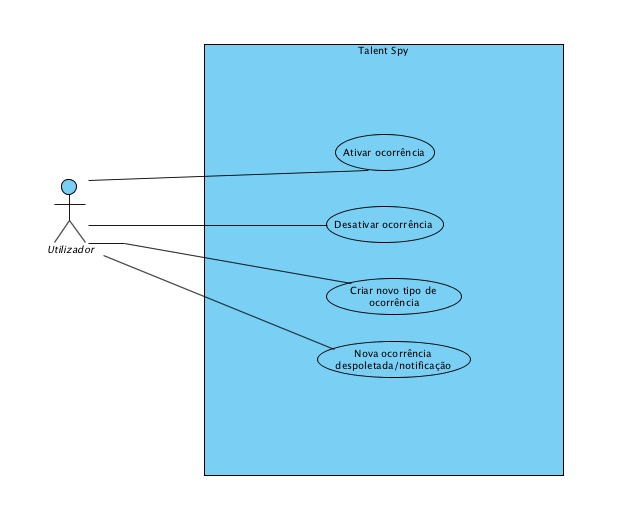
\includegraphics[scale=0.6]{img/er.jpg}
    \caption{Diagrama de \emph{Use Cases}}
    \label{fig:use cases}
\end{figure}

\subsection{Especificações dos \emph{Use Cases} do Produto}

Nesta secção iremos especificar cada um dos \emph{Use Cases} detetados. Esta especificação passa por definir os atores que entrevem no \emph{Use Case}, uma descrição do \emph{Use Case}, os dados com que o \emph{Use Case} lida, o estímulo que inicia o \emph{Use Case}, a resposta do sistema e possivelmente algum comentário extra.

\subsubsection{\emph{Use Case} 1: Ativar ocorrência}
\begin{table}[H]
\centering
\label{my-label}
\begin{tabular}{|l|p{320pt}|}
\hline
Atores      & Utilizador                                                                                                                                                                                                        \\ \hline
Descrição   & O utilizador pode ativar ocorrências para receber notificações de um determinado aspeto do jogador.  \\ \hline
Dados       & Dados dos Jogadores e Tipo de ocorrência                                                                                                                                                                                                          \\ \hline
Estímulo    & Pedido realizado pelo utilizador.                                                                                                                                                                                            \\ \hline
Resposta    & \begin{tabular}[c]{@{}l@{}}É criada uma nova ocorrência e o sistema refere que o \\ utilizador em questão quer receber notificações quando a \\ pré-condição da ocorrência for atingida.\end{tabular}                                                                                    \\ \hline
Comentários & Existe um historial de ocorrências ativadas e desativadas.                                                                                                                                                                 \\ \hline
\end{tabular}
\end{table}

\subsubsection{\emph{Use Case 2}: Desativar ocorrência}
\begin{table}[H]
\centering
\label{my-label}
\begin{tabular}{|l|p{320pt}|}
\hline
Atores      & Utilizador                                                                                                                                                                                                       \\ \hline
Descrição   & O utilizador pode, a qualquer momento, desativar uma ocorrência para um determinado jogador que tenha ativado previamente. \\ \hline
Dados       & Dados dos Jogadores e Histórico de Ocorrências.                                                                                                                                                                                                          \\ \hline
Estímulo    & Pedido realizado pelo utilizador.                                                                                                                                                                                            \\ \hline
Resposta    & \begin{tabular}[c]{@{}l@{}}A ocorrência é removida e o utilizador deixa de receber\\ notificações para a ocorrência removida.\end{tabular}                                                                                    \\ \hline
Comentários & A ocorrência é mantida no historial de ocorrências mas com o estado desativada.                                                                                                                                                                 \\ \hline
\end{tabular}
\end{table}


\subsubsection{\emph{Use Case 3}: Adicionar novo tipo ocorrência}
\begin{table}[H]
\centering
\label{my-label}
\begin{tabular}{|l|p{320pt}|}
\hline
Atores      & Utilizador                                                                                                                                                                                                        \\ \hline
Descrição   & O utilizador pode adicionar novas ocorrências ao sistema complementando as já existentes.  \\ \hline
Dados       & Dados da nova ocorrência.                                                                                                                                                                                                          \\ \hline
Estímulo    & Pedido realizado pelo utilizador.                                                                                                                                                                                            \\ \hline
Resposta    & \begin{tabular}[c]{@{}l@{}}A ocorrência é adicionada e o sistema apresenta\\ uma mensagem de sucesso ou insucesso.\end{tabular}                                                                                    \\ \hline
Comentários & As ocorrências contemplam agora as hipóteses adicionadas.                                                                                                                                                                 \\ \hline
\end{tabular}
\end{table}

\subsubsection{\emph{Use Case 4}: Alertar utilizar de pré-condição de ocorrência atingida}
\begin{table}[H]
\centering
\label{my-label}
\begin{tabular}{|l|p{320pt}|}
\hline
Atores      & Utilizador                                                                                                                                                                                                        \\ \hline
Descrição   & A pré-condição de uma ocorrência ativa pelo utilizador é atingida e o utilizador é alertado pela aplicação móvel e/ou por SMS. \\ \hline
Dados       & Dados dos Jogadores e Ocorrências ativas.                                                                                                                                                                                                         \\ \hline
Estímulo    & Ação despoletada pelo sistema.                                                                                                                                                                                            \\ \hline
Resposta    & \begin{tabular}[c]{@{}l@{}}O utilizador recebe uma notificação na aplicação e/ou SMS.\end{tabular}                                                                                    \\ \hline
Comentários &  O utilizador só recebe um SMS com os dados caso tenha ativado a opção.                                                                                                                                                              \\ \hline
\end{tabular}
\end{table}

\section{Requisitos Funcionais}

\subsection{Requisitos Funcionais}

Nos requisitos vamos usar uma técnica de priorização chamada de agrupamento \emph{MoSCoW}. Esta técnica divide-se em quatro partes, sendo cada uma identificada com uma letra:
\begin{itemize}
\item \emph{\textbf{M}ust}: requisitos que têm de ser considerados.
\item \emph{\textbf{S}hould}: requisitos que devem ser considerados.
\item \emph{\textbf{C}ould}: requisitos desejáveis mas não necessários.
\item \emph{\textbf{W}on’t}: requisitos que poderão ser considerados no futuro.
\end{itemize}

\newpage

\begin{framed}
\noindent\textbf{Requisito no:} 1
\qquad
\textbf{\emph{Use case} no:} 4
\vspace{2mm}
\newline\textbf{Descrição:} O produto deve notificar os utilizadores quando a pré-condição de uma ocorrência por si ativada é atingida.
\vspace{1mm}
\newline\textbf{Razão/Motivação:} Notificar o utilizador.
\vspace{1mm}
\newline\textbf{Criador:} Rogério Moreira, Rúben Santos, Pedro Vital (\emph{F3M})
\vspace{1mm}
\newline\textbf{Critério de encaixe:} Quando a pré-condição de uma ocorrência é atingida o utilizador terá que ser notificado e ter a noção de qual foi.
\vspace{1mm}
\newline\textbf{Prioridade:} M
\vspace{1mm}
\newline\textbf{Data:} 16/11/2017
\end{framed}

\begin{framed}
\noindent\textbf{Requisito no:} 2
\qquad
\textbf{\emph{Use case} no:} 4
\vspace{2mm}
\newline\textbf{Descrição:} Os utilizadores devem ser capazes de ver as notificações recebidas passadas e atuais na aplicação móvel e no portal \emph{TalentSpy}.
\vspace{1mm}
\newline\textbf{Razão/Motivação:} Ter um histórico das notificações.
\vspace{1mm}
\newline\textbf{Criador:} Rogério Moreira, Rúben Santos, Pedro Vital (\emph{F3M}), Tiago Sá
\vspace{1mm}
\newline\textbf{Critério de encaixe:} Os utilizadores devem ter a perceção do histórico das notificações.
\vspace{1mm}
\newline\textbf{Prioridade:} M
\vspace{1mm}
\newline\textbf{Data:} 16/11/2017
\end{framed}

\newpage

\begin{framed}
\noindent\textbf{Requisito no:} 3
\qquad
\textbf{\emph{Use case} no:} 3
\vspace{2mm}
\newline\textbf{Descrição:} Os utilizadores devem ser capazes de criar novos tipos de ocorrências baseadas num conjunto de pré-condições e dados.
\vspace{1mm}
\newline\textbf{Razão/Motivação:} Alargar o âmbito do sistema.
\vspace{1mm}
\newline\textbf{Criador:} Rogério Moreira, Pedro Vital (\emph{F3M})
\vspace{1mm}
\newline\textbf{Critério de encaixe:} Caso não estejam satisfeitos com nenhum tipo de ocorrência disponíveis na plataforma devem ser capazes de criar novos tendo em conta os dados disponíveis de cada jogador.
\vspace{1mm}
\newline\textbf{Prioridade:} S
\vspace{1mm}
\newline\textbf{Data:} 20/12/2017
\end{framed}

\begin{framed}
\noindent\textbf{Requisito no:} 4
\qquad
\textbf{\emph{Use case} no:} 1
\vspace{2mm}
\newline\textbf{Descrição:} Os utilizadores terão uma lista pré-definida de tipos de ocorrências que podem ativar para um determinado jogador.
\vspace{1mm}
\newline\textbf{Razão/Motivação:} Âmbito do sistema
\vspace{1mm}
\newline\textbf{Criador:} Rogério Moreira, Tiago Sá, Samuel Ferreira, Rúben Santos
\vspace{1mm}
\newline\textbf{Critério de encaixe:} A partir da lista pré-definida os utilizadores podem ativar qualquer tipo de ocorrência para um determinado jogador, facilitando o trabalho inicial.
\vspace{1mm}
\newline\textbf{Prioridade:} M
\vspace{1mm}
\newline\textbf{Data:} 13/10/2017
\end{framed}

\newpage
\begin{framed}
\noindent\textbf{Requisito no:} 5
\vspace{2mm}
\newline\textbf{Descrição:} O utilizador deve autenticar-se no portal \emph{TalentSpy}.
\vspace{1mm}
\newline\textbf{Razão/Motivação:} Autenticação do sistema
\vspace{1mm}
\newline\textbf{Criador:} Rogério Moreira, Tiago Sá, Pedro Vital (\emph{F3M}), Rúben Santos
\vspace{1mm}
\newline\textbf{Critério de encaixe:} Os utilizadores devem ter uma conta no \emph{TalentSpy} com \emph{login} válido para poderem gerir as ocorrências.
\vspace{1mm}
\newline\textbf{Prioridade:} M
\vspace{1mm}
\newline\textbf{Data:} 13/10/2017
\end{framed}

\begin{framed}
\noindent\textbf{Requisito no:} 6
\qquad
\textbf{\emph{Use case} no:} 2
\vspace{2mm}
\newline\textbf{Descrição:} Os utilizadores devem ser capazes de eliminar as notificações de um certo tipo de ocorrência.
\vspace{1mm}
\newline\textbf{Razão/Motivação:} Deixar de ser notificado
\vspace{1mm}
\newline\textbf{Criador:} Rogério Moreira
\vspace{1mm}
\newline\textbf{Critério de encaixe:} Quando um tipo de ocorrência já não é útil então deve poder ser eliminada pelo utilizador.
\vspace{1mm}
\newline\textbf{Prioridade:} C
\vspace{1mm}
\newline\textbf{Data:} 23/12/2017
\end{framed}

\newpage

\begin{framed}
\noindent\textbf{Requisito no:} 7
\qquad
\textbf{\emph{Use case} no:} 1, 2
\vspace{2mm}
\newline\textbf{Descrição:} Os utilizadores devem ser capazes de ativar um tipo de ocorrência pré-definida ou por si definida.
\vspace{1mm}
\newline\textbf{Razão/Motivação:} Ter o controlo das notificações recebidas
\vspace{1mm}
\newline\textbf{Criador:} Rogério Moreira, Samuel Ferreira, Tiago Sá, Rúben Santos
\vspace{1mm}
\newline\textbf{Critério de encaixe:} Os utilizadores poderão a qualquer momento ativar ou desativar uma ocorrência para um determinado jogador.
\vspace{1mm}
\newline\textbf{Prioridade:} S
\vspace{1mm}
\newline\textbf{Data:} 23/12/2017
\end{framed}

\begin{framed}
\noindent\textbf{Requisito no:} 8
\vspace{2mm}
\newline\textbf{Descrição:} Os utilizadores devem poder exportar as ocorrências por si criadas, bem como os jogadores às quais estavam associadas.
\vspace{1mm}
\newline\textbf{Razão/Motivação:} Mudança de conta
\vspace{1mm}
\newline\textbf{Criador:} Rogério Moreira
\vspace{1mm}
\newline\textbf{Critério de encaixe:} Quando existe uma mudança de conta (uma conta é encerrada ou a pessoa responsável muda) então deve ser possível exportar os dados para a nova conta.
\vspace{1mm}
\newline\textbf{Prioridade:} C
\vspace{1mm}
\newline\textbf{Data:} 05/01/2018
\end{framed}

\newpage

\begin{framed}
\noindent\textbf{Requisito no:} 9
\qquad
\vspace{2mm}
\newline\textbf{Descrição:} Os utilizadores devem poder importar as ocorrências e estas deverão voltar a ficar ativas.
\vspace{1mm}
\newline\textbf{Razão/Motivação:} Mudança de conta
\vspace{1mm}
\newline\textbf{Criador:} Rogério Moreira
\vspace{1mm}
\newline\textbf{Critério de encaixe:} Quando existe uma mudança de conta (uma conta é encerrada ou a pessoa responsável muda) então deve ser possível exportar os dados para a nova conta.
\vspace{1mm}
\newline\textbf{Prioridade:} C
\vspace{1mm}
\newline\textbf{Data:} 05/01/2018
\end{framed}

\begin{framed}
\noindent\textbf{Requisito no:} 10
\qquad
\vspace{2mm}
\newline\textbf{Descrição:} Os utilizadores devem ser capazes de ver uma lista de todas as ocorrências ativas para a sua conta.
\vspace{1mm}
\newline\textbf{Razão/Motivação:} Ver o historial de ocorrências
\vspace{1mm}
\newline\textbf{Criador:} Rogério Moreira
\vspace{1mm}
\newline\textbf{Critério de encaixe:} Ter uma perceção de todas as ocorrências.
\vspace{1mm}
\newline\textbf{Prioridade:} C
\vspace{1mm}
\newline\textbf{Data:} 05/01/2018
\end{framed}

\newpage

\begin{framed}
\noindent\textbf{Requisito no:} 11
\vspace{2mm}
\newline\textbf{Descrição:} Os utilizadores, para usufruir do serviço, terão que ter uma conta válida na plataforma \emph{Talent Spy}.
\vspace{1mm}
\newline\textbf{Razão/Motivação:} A licença para uso deste sistema é a mesma da plataforma \emph{TalentSpy}.
\vspace{1mm}
\newline\textbf{Criador:} Rogério Moreira, Samuel Ferreira
\vspace{1mm}
\newline\textbf{Prioridade:} M
\vspace{1mm}
\newline\textbf{Data:} 09/01/2018
\end{framed}
